% Use only LaTeX2e, calling the article.cls class and 12-point type.

\documentclass[12pt]{article}

% Users of the {thebibliography} environment or BibTeX should use the
% scicite.sty package, downloadable from *Science* at
% www.sciencemag.org/about/authors/prep/TeX_help/ .
% This package should properly format in-text
% reference calls and reference-list numbers.

\usepackage{scicite}
\usepackage{graphicx}
% Use times if you have the font installed; otherwise, comment out the
% following line.

\usepackage{times}

% The preamble here sets up a lot of new/revised commands and
% environments.  It's annoying, but please do *not* try to strip these
% out into a separate .sty file (which could lead to the loss of some
% information when we convert the file to other formats).  Instead, keep
% them in the preamble of your main LaTeX source file.


% The following parameters seem to provide a reasonable page setup.

\topmargin 0.0cm
\oddsidemargin 0.2cm
\textwidth 16cm 
\textheight 21cm
\footskip 1.0cm


%The next command sets up an environment for the abstract to your paper.

\newenvironment{sciabstract}{%
\begin{quote} \bf}
{\end{quote}}


% If your reference list includes text notes as well as references,
% include the following line; otherwise, comment it out.

\renewcommand\refname{References and Notes}

% The following lines set up an environment for the last note in the
% reference list, which commonly includes acknowledgments of funding,
% help, etc.  It's intended for users of BibTeX or the {thebibliography}
% environment.  Users who are hand-coding their references at the end
% using a list environment such as {enumerate} can simply add another
% item at the end, and it will be numbered automatically.

\newcounter{lastnote}
\newenvironment{scilastnote}{%
\setcounter{lastnote}{\value{enumiv}}%
\addtocounter{lastnote}{+1}%
\begin{list}%
{\arabic{lastnote}.}
{\setlength{\leftmargin}{.22in}}
{\setlength{\labelsep}{.5em}}}
{\end{list}}


% Include your paper's title here

\title{Homework 3} 


% Place the author information here.  Please hand-code the contact
% information and notecalls; do *not* use \footnote commands.  Let the
% author contact information appear immediately below the author names
% as shown.  We would also prefer that you don't change the type-size
% settings shown here.

\author
{NAME: Kuangyi Yang\\
ID: A53083212\\
LOGIN: cs12fig
}


% Include the date command, but leave its argument blank.

\date{}



%%%%%%%%%%%%%%%%% END OF PREAMBLE %%%%%%%%%%%%%%%%



\begin{document} 

% Double-space the manuscript.

\baselineskip24pt

% Make the title.

\maketitle 




% In setting up this template for *Science* papers, we've used both
% the \section* command and the \paragraph* command for topical
% divisions.  Which you use will of course depend on the type of paper
% you're writing.  Review Articles tend to have displayed headings, for
% which \section* is more appropriate; Research Articles, when they have
% formal topical divisions at all, tend to signal them with bold text
% that runs into the paragraph, for which \paragraph* is the right
% choice.  Either way, use the asterisk (*) modifier, as shown, to
% suppress numbering.

\section*{ Part 1A}
1. False
\\2. True
\\3. False
\\4. False
\\5. True
\\6. True
\\7. False
\\8. True
\\9. False
\\10. True
\\11. False
\\12. False
\\13. True
\\14. True
\\15. False

\section*{Part 1B}
11. $f(n) = n^2-100n-1000$ is a $O(n^2)$ function, $g(n) = n$ is a $O(n)$ function
There is no way to pick a c that would make an $O(n)$ function stay above an 
$O(n^2)$ function, so in this problem, we only have $f(n) = \Omega(g(n))$, $f(n) = O(g(n))$
is false, so $f(n) = \Theta(g(n))$ is false.\\
\\
12. $f(n) = n^2-4n-4$ is a $O(n^2)$ function, $g(n) = n^3$ is a $O(n^3)$ function
There is no way to pick a c that would make an $O(n^2)$ function stay above an 
$O(n^3)$ function, so in this problem, we only have $f(n) = O(g(n))$, $f(n) = \Omega(g(n))$
is false, so $f(n) = \Theta(g(n))$ is false.\\
\\
13. let $f(n) = 100n + \sqrt n + 4$ and $g(n) = n$, we can find $c = 101$ and $n_0 = 6$, such that $f(n) \leq cg(n)$ for $n \geq n_0$, so $f(n) = O(g(n))$. \\
We can also find $c = 1$ and $n_0 = 1$,such that $f(n) \geq cg(n)$ for $n \geq n_0$, so $f(n) = \Omega(g(n))$. 
\\Since $f(n) = O(g(n))$ and $f(n) = \Omega(g(n))$, then $f(n) = \Theta(g(n))$\\
\\
14. let $f(n) = 2n*n + 10n + 100$ and $g(n) = n^2$, we can find $c = 3$ and $n_0 = 17$, such that $f(n) \leq cg(n)$ for $n \geq n_0$, so $f(n) = O(g(n))$. \\
We can also find $c = 1$ and $n_0 = 1$,such that $f(n) \geq cg(n)$ for $n \geq n_0$, so $f(n) = \Omega(g(n))$. 
\\Since $f(n) = O(g(n))$ and $f(n) = \Omega(g(n))$, then $f(n) = \Theta(g(n))$\\
\\
15. $f(n) = n^2+log(n)*n^2$ is a $O(n^2log(n))$ function, $g(n) = n^2$ is a $O(n^2)$ function
There is no way to pick a c that would make an $O(n^2)$ function stay above an 
$O(n^2log(n))$ function, so in this problem, we only have $f(n) = \Omega(g(n))$, $f(n) = O(g(n))$
is false, so $f(n) = \Theta(g(n))$ is false.\\

\section*{Part 2}
1) Running time: $O(n)$\\
Explanation: There is a single loop that runs (2*n-1+1) times. Each time the loop runs it executes 1 instruction, so the goal number  of instructions executed is $1*(2*n-1+1) = O(2n) = O(n)$\\
\\
2) Running time: $O(n^2)$\\
Explanation: There is a single loop that runs $(n^2-1+1)$ times. Each time the loop runs it executes 1 instruction, so the goal number  of instructions executed is $1*(n^2-1+1) = O(n^2)$\\
\\
3) Running time: $O(n)$\\
Explanation: There is a single loop that runs $(n-1+1)$ times. Each time the loop runs it executes 1 instruction, so the goal number  of instructions executed is $1*(n-1+1) = O(n)$\\
\\
4) Running time: $O(n^2)$\\
Explanation: There is an outer loop that runs $n$ times. Each time the loop runs it executes a inner loop, each inner loop runs $i$ times, $i = 1,2,....,n$, each time the inner loop runs it executes 1 instruction. so the goal number  of instructions executed is $1*(1+2+...+n) = O(\frac{1}{2}n^2+\frac{1}{2}) = O(n^2)$\\
\\
5) Running time: $O(n)$\\
Explanation: There is an outer loop that runs 100 times. Each time the loop runs it executes a inner loop, each inner loop runs $n$ times, each time the inner loop runs it executes 1 instruction. so the goal number  of instructions executed is $1*100*n = O(100n) = O(n)$\\
\\
6) Running time: $O(nlog_2n)$\\
Explanation: There is an outer loop that runs $n$ times. Each time the loop runs it executes a inner loop, each inner loop runs $log_{2}n$ times, each time the inner loop runs it executes 1 instruction. so the goal number  of instructions executed is $1*n*log_{2}n = O(nlog_2n)$\\
\\
7) Running time: $O(n)$\\
Explanation: There are two loops without nested, the first loop runs $n$ times. Each time the loop runs it executes 1 instruction, the second loop runs $2n+1$ times, each time the loop runs it executes 1 instruction. so the goal number of instructions executed is $1*n + 1*(2n+1) = O(3n+1) = O(n)$\\
\\
8) Running time: $O(1)$\\
Explanation: There is a single loop that runs 500 times. Each time the loop runs it executes 1 instruction, so the goal number  of instructions executed is $1*500 = O(500) = O(1)$\\
\\
9) Running time: $O(n)$\\
Explanation: There is a single loop that runs $n$ times. Each time the loop runs it executes 3 instruction, so the goal number  of instructions executed is $3*n = O(3n) = O(n)$\\
\\
10) Running time: $O(n^2)$\\
Explanation: There are two loops, the first outer loop contains a inner loop. The first loop runs $n$ times. Each time the loop runs it executes a inner loop, each inner loop runs $n$ times, each time the inner loop runs it executes 1 instruction. The second loop runs $n$ times, each time the loop runs it executes 1 instruction. so the goal number of instructions executed is $1*n*n + 1*n= O(n^2 + n) = O(n^2)$\\
\\
\section*{Part 3}
\begin{figure}[h!]
  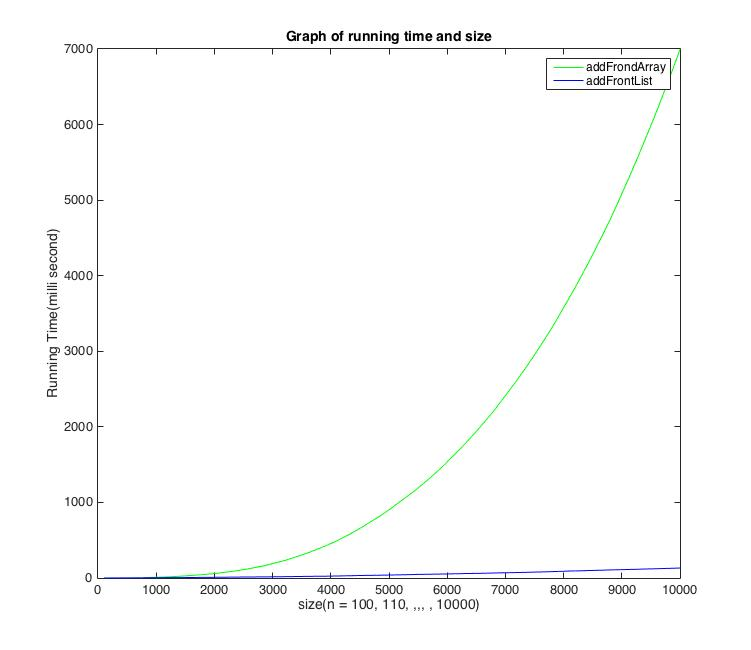
\includegraphics[width=\linewidth]{hw3.jpg}
  \caption{Graph of Running time and Size}
  \label{fig:Running Time}
\end{figure}

~~\\
Based on the experiments, running time of addFrontArray is quadratic to size of array n, so time complexity of method addFrontArray is $O(n^2)$; This is because when we add n numbers to the front of the array, one by one, there is an outer loop, and this outer loop runs n times, when we add each number to the front of the array, we need to shift the rest numbers in the array, there is an inner loop, and this inner loop runs $n-1$ times for shifting, so complexity is $n*(n-1) = O(n^2)$.\\
Based on the experiments, running time of addFrontList is linear to size of list n, so time complexity of method addFrontArray is $O(n)$; This is because when we add n numbers to the from of the list, one by one, there is a loop, which runs n times. Each time the loop runs it executes 1 instruction to add the from element. So the goal number of instructions executed is $1*n = O(n)$.
\\

\end{document}




















